\chapter{Semi Automatic Annotation} \label{chapter:semi_automatic}

\begin{figure}[!tbp]
	\centering
    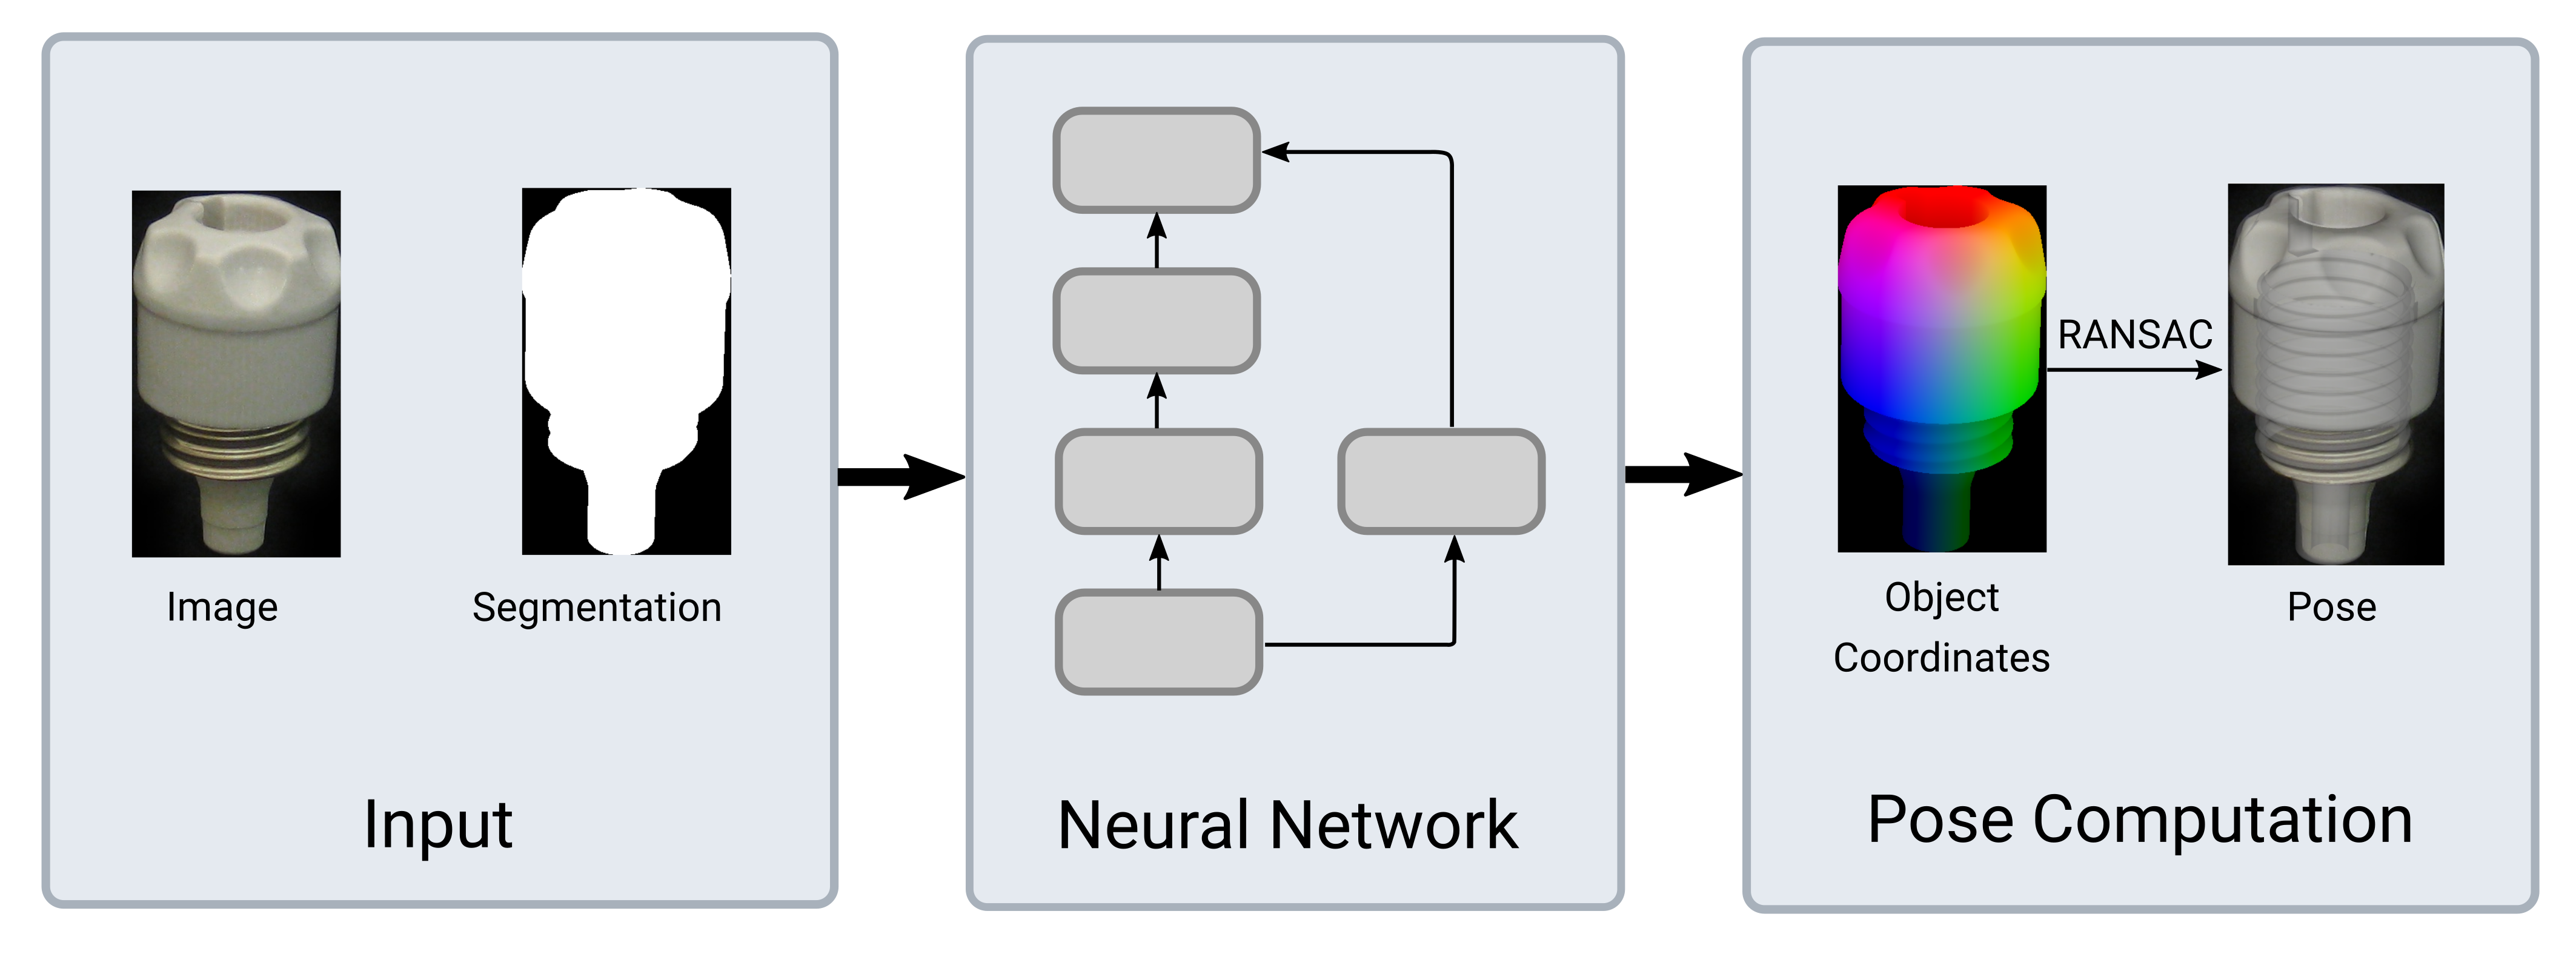
\includegraphics[width=\linewidth]{network_pipeline}
    \caption{The pipeline of the neural network. The two inputs of the network are the image and the corresponding segmentation image. The neural network then uses the segmentation to retrieve the pixels to predict object coordinates for. In the final pose computation stage the object coordinates and their 2D locations are used to retrieve the best pose using RANSAC.}
    	\label{fig:network_pipeline}
\end{figure} 

To assist in the process of manual image annotation presented in Chapter \ref{chapter:manual_annotation}, we developed a neural network for the task of 6D pose estimation tailored to the characteristics of the images of the Endoscopic Vision Challenge. This chapter describes the network architecture and its variations, as well as different approaches to train the network and the resulting modified annotation procedure.

\section{Terminology} \label{section:network_terminology}

\noindent\textbf{Residual Connection.} A \textit{residual connection} (or \textit{skip connection}) is a part of a neural network that skips some layers of the network and adds the input of a layer to the output of a layer that is situated deeper in the network. They can prevent the problem of the increasing training error in deeper networks \cite{resnet}. Fig. \ref{fig:residual_connection} visualizes such a connection. \\

\noindent\textbf{Training Set.} A \textit{training set} is a subset of the dataset intended to train a neural network with. The training set is the set that the network actually uses to adjust its weights as opposed to the validation set. \\

\noindent\textbf{Training Example.} A \textit{training example} is an element from the training set fed to the neural network during training. \\

\noindent\textbf{Training Batch.} A \textit{training batch} consists of a subset of training examples. During training the network updates its weights using all examples in the batch. \\

\noindent\textbf{Validation Set.} A \textit{validation set} is a subset of the dataset intended to train a neural network with. The validation set's purpose is to validate the network's new configuration which emerged from a run within the training. \\

\noindent\textbf{L1 Loss.} The \textit{L1 loss} is a loss function that sums up the results of the function $g$ applied to the $k$ elements in a training batch, i.e. $L_1(x, y) = \sum\limits_k |g(x_k, y_k)|$. The function $g(x, y)$ can be arbitrary, in our case we set it to the euclidean distance $g(x, y) = \sqrt{\sum\limits_i (x_i - y_i)^2}$, $x_i$ and $y_i$ being the entries of the vectors $x$ and $y$, respectively. \\

\noindent\textbf{L2 Loss.} The \textit{L2 loss} is a loss function defined similarly to the L1 loss but sums up the squared instead of the absolute results of $g$, i.e. $L_2(x, y) = \sum\limits_i g(x_i - y_i)^2$. \\

\noindent\textbf{L2 Regularization.} \textit{L2 regularization} penalizes the weights by a factor $\lambda$ in the following way: $\lambda \sum\limits_i w_i^2$. The regularization term is added to the weight update to keep the network from overfitting. \\

\noindent\textbf{Dropout Percentage.} \textit{Dropout percentage} is the percentage of neurons to deactivate in a layer during training. \\

\noindent\textbf{Receptive Field-Size.} The \textit{receptive field-size} of a network denotes how many input pixels an output value of the network has taken into account. This factor is determined by the number of operations in the network and their parameters. A convolution operation can skip pixels and the size of the layer's kernel can be adjusted, which both result in a larger receptive field-size. Depending on the field of application a field-size should be larger or smaller.

\section{Implementation}

The neural network and all of its utility functionality is implemented in Python using Tensorflow \cite{tensorflow} and Keras \cite{keras}. Tensorflow is a deep-learning framework that uses C++ do perform the actual calculations. It provides many different layers, as well as tools to modify images, automatic differentiation of the loss function and a lot of other functionality. Keras is a framework that makes using Tensorflow easier by providing even higher-level access and allows to create neural network in a few lines of code. Because most operations of a neural network written in Tensorflow and Keras are performed using C++ code and because computation can be transferred to the GPU at nearly no extra effort, such a network is considerably faster than an implementation in Python might imply.

\section{Network Architecture}

The architecture of the network is adjusted to the problem domain of the images of the Endoscopic Vision Challenge. There is no mechanism of inferring the masks and the network expects RGB-only images without depth. This significantly reduces the complexity of predicting the position of the object. Heavily contradicting object coordinates can still lead to positional errors. This precondition gave rise to the pipeline shown in \fig \ref{fig:network_pipeline} which takes the actual image and the segmentation image as input. The images shown are already cropped to the segmentation mask but in later applications the image size and proportion of pixels belonging to the object can be arbitrary. The network processes each pixel which is part of the object according to the segmentation image and outputs the 3D coordinates. As explained in Chapter \ref{chapter:background}, we then compute the optimal pose using RANSAC and the 2D-3D correspondences.

The basic architecture that we chose for the network is called ResNet. ResNet was first presented in \cite{resnet} and enabled researchers to create deeper networks than before. Two major problems arise with very deep neural networks. The vanishing gradients problem, which means that gradients gradually become 0 in deeper layers. This can problem be targeted with batch normalization. Making a network deeper without further adjustments can lead to an increasing training eror. Adding layers to a network to increase expressivity does not directly lead to a higher accuracy. Even stacking identity layers, i.e. layers that learn the mathmatical identity function $f(x) = x$, ontop of the network increases the training error. This phenomenom can be partly compensated with residual connections \cite{resnet}. An example of a residual connection can be seen in \fig \ref{fig:residual_connection}. Fig. \ref{fig:resnet_comparison} shows a comparison of ResNet with the architecture \textit{VGG} \cite{vgg}. The residual connections are clearly visible as the arcs of the rightmost architecture.

\begin{figure}[!tbp]
	\centering
	\begin{subfigure}[t]{0.47\textwidth}
		\centering
    	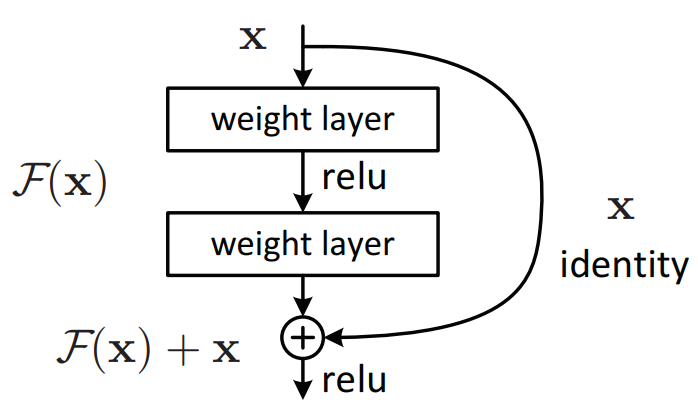
\includegraphics[width=\linewidth]{residual_connection}
    	\caption{A detailed view on a residual connection. The residual connections add the input of earlier layers of the network to deeper ones.}
    	\label{fig:residual_connection}
	\end{subfigure}
	\hfill
	\begin{subfigure}[t]{0.47\textwidth}
		\centering
    	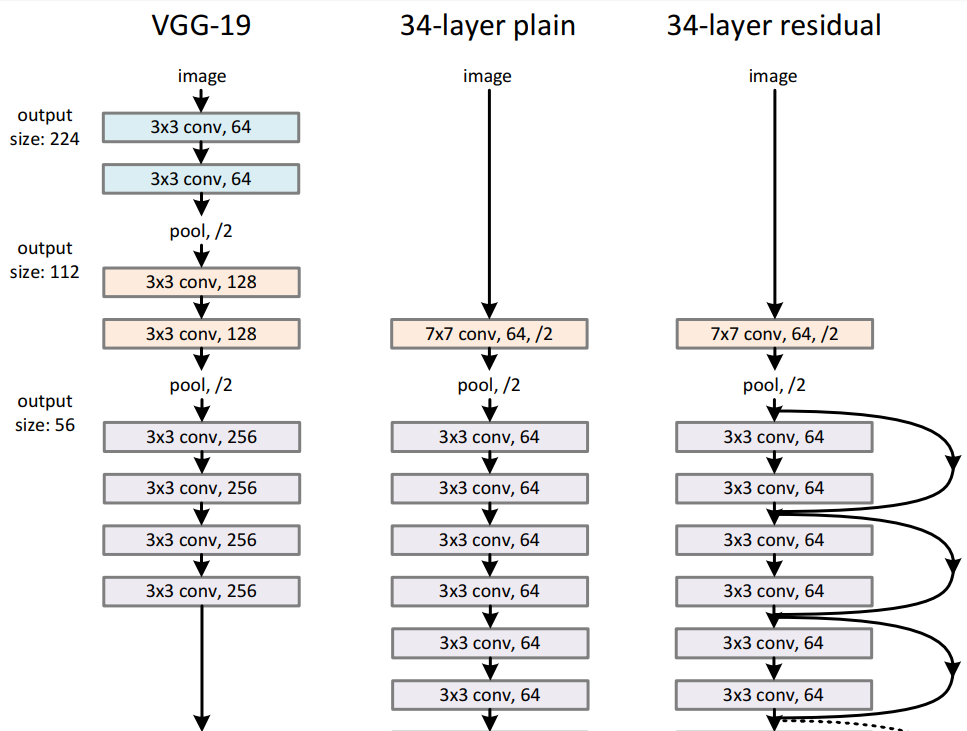
\includegraphics[width=\linewidth]{resnet_comparison}
    	\caption{Excerpt of a comparison between the ResNet architecture and VGG. The ResNet allows the creation of deeper network as the problem of vanishing gradients, i.e. very small gradients at deeper layers, can be targeted this way. The image has been cropped.}
    	\label{fig:resnet_comparison}
	\end{subfigure}
	\caption{A key component of ResNet: the residual connection. Left shows the connection in detail and right shows a comparison with the VGG architecture. Images from \cite{resnet}.}
	\label{fig:resnet_details}
\end{figure} 

The structure of the network is visualized in \fig \ref{fig:network_architecture}. The depicted version has 23 convolutional layers. The building blocks of the network are the \textit{Conv Block} and the \textit{ID Block}. Both blocks are shown in detail on the right. A Conv Block applies another convolution to the shortcut connection on the right and then combines the result with the output of the left path. The ID Block simply adds the input to the output of the left path. The figure doesn't show the batch normalization and \textit{activation layers} to keep the illustration clear. The actual network has a batch normalization layer after each convolution layer and an activation layer after each batch normalization layer. Activation layers are layers in Keras that apply a specified activation function to their input. This is how non-linear neurons are realized in the framework.

\subsection{Loss \& Optimizer}

Since the network outputs the 3D coordinates for each pixel in the input image a straight-forward approach is to penalize the euclidean distance with respect to the ground-truth coordinates. The loss function sums up the absolute distances of the individual XYZ components of the predicted object coordinate and the ground-truth, but only at the relevant positions according to the segmentation mask. This resembles the L1 loss (see Section \ref{section:network_terminology}). The reason why we chose the L1 loss over the L2 loss is that the L2 loss penalizes outliers more. Outliers will already get eliminated in the \gls{ransac} algorithm during pose computation. The L2 loss might strive for a worse compromise. We used L2 regularization of the weights. We compared SGD and Adam to find the best optimizer for the network (see Chapter \ref{chapter:background} for details on the optimizers).

\begin{figure}[!tbp]
	\centering
    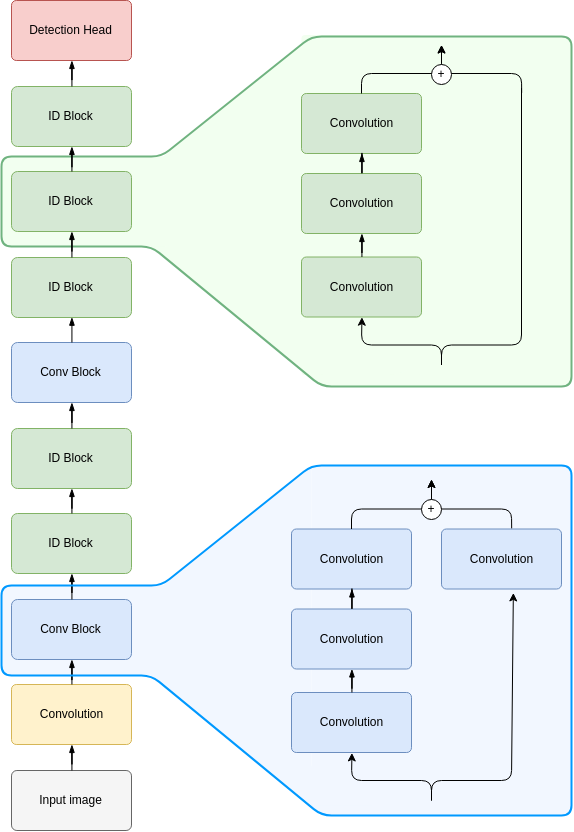
\includegraphics[width=0.9\linewidth]{flowerpower_short}
    \caption{Architecture 1 with a total of 23 (convolutional) layers. The components of the \textbf{Conv Block} and \textbf{ID Block} elements are visualized on the right. The characteristic of the Conv Block is that it applies a convolution on the shortcut connection, while the ID Block doesn't. The yellow \textbf{Convolution} rectangle is a plain convolution layer. The \textbf{Detection Head} consists of another three convolution layers. Own image.}
    	\label{fig:network_architecture}
\end{figure}

\subsection{Variations} \label{section:network_variations}

\begin{table}[]
\centering
\begin{tabular}{|l||llllll|}
\hline Architecture No.        & 1          & 2          & 3          & 4          & 5          & 6        \\ \hline\hline
\rowcolor{Gray}
\# Layers               & 23         & 35         & 23         & 50         & 50         & 50       \\
Receptive field-size    & 99         & 67         & 51         & 59         & 59         & 59       \\
\rowcolor{Gray}
\# Parameters & 3,95M  & 19,69M & 6,32M  & 24,63M & 24,63M   & 24,63M \\
Data normalization      & bn & bn & bn & do    & bn & do \\ \hline
\end{tabular}
\caption{Overview over the differences of the network architectures. The number of layers corresponds to the number of convolutional layers. Batch normalization layers are not counted. The abbreviations "bn" and "do" stand for batch normalization and dropout, respectively. The number of parameters is given in millions. Parameters are trainable variables of the network. The number of parameters does not scale linearly with the number of layers as deeper layers have more filters in the network. Own table.}
\label{table:network_architectures}
\end{table}

To find the optimal network structure a total of 6 network architectures were created and later compared in Chapter \ref{chapter:experiments}. The first design of the network consisted of 23 convolutional layers with a receptive field-size of 99. A characteristic of the Endoscopic Vision Challenge dataset is that the tools have writings on them which is often not or only partly visible. To keep the network from detecting poses mainly based on the letters, we reduced the receptive field-size for the other architectures. We enlarged the second architecture to a total of 35 layers, while decreasing the receptive field-size to 67. The third architecture kept the number of layers of the first but reduced the field-size to 51. Architectures 4 to 6 all have a receptive field-size of 59 and the 50 convolutional layers. While architecture 5 uses batch normalization for regularization, the architectures 4 and 5 use dropout instead. The difference between those two is the dropout percentage. An overview over the architectures can be seen in Table \ref{table:network_architectures}.

\section{Modes of Operation} \label{section:modes_of_operation}

The goal of the neural network is to make the annotation process presented in chapter \ref{chapter:manual_annotation} faster and more efficient. To achieve this we strove for a symbiosis between the annotation tool and the neural network. The new workflow is visualized in \fig \ref{fig:semi_automatic_workflow}. In addition to manually annotating images, the user train the network with the data. After training the neural network, the user can run the network on unseen images to predict poses and correct them with the aid of the annotation tool. The improved pose predictions can serve as input to further train the network. There are two main strategies of training a neural network that we will consider here. Those two are training from scratch and an incremental training approach.

\noindent\textbf{Training from Scratch.} \textit{Training from scratch} describes the method of training the network with all images (usually divided into training and validation set) and initializing  the weights of the network to 0 or random values. This procedure requires a lot of time as many images have to be processed. It also requires many already annotated training examples.

\noindent\textbf{Incremental Training.} \textit{Incremental training} is the procedure of not training the network from scratch each time a sufficient amount of new images has been annotated. Instead, the network is trained with fewer images first. Then, while the user annotates more images, the network is trained again using the weights that were obtained in the previous training process. These steps are repeated constantly during the annotation process. Each single training run finished faster than the training runs when training from scratch, as there are less images to train the network with. A question that arises is whether training from scratch and incremental training achieve similar results, or one outperforms the other.

\noindent\textbf{Inference.}  After training the network using one of the two training strategies, it can be used to predict poses on unseen images. To amortize the time needed to load the weights of the network it is best to run inference for many images and not only one. The network inference can be directly called from the annotation tool that we presented in chapter \ref{chapter:manual_annotation}.

\begin{figure}[!tbp]
	\centering
    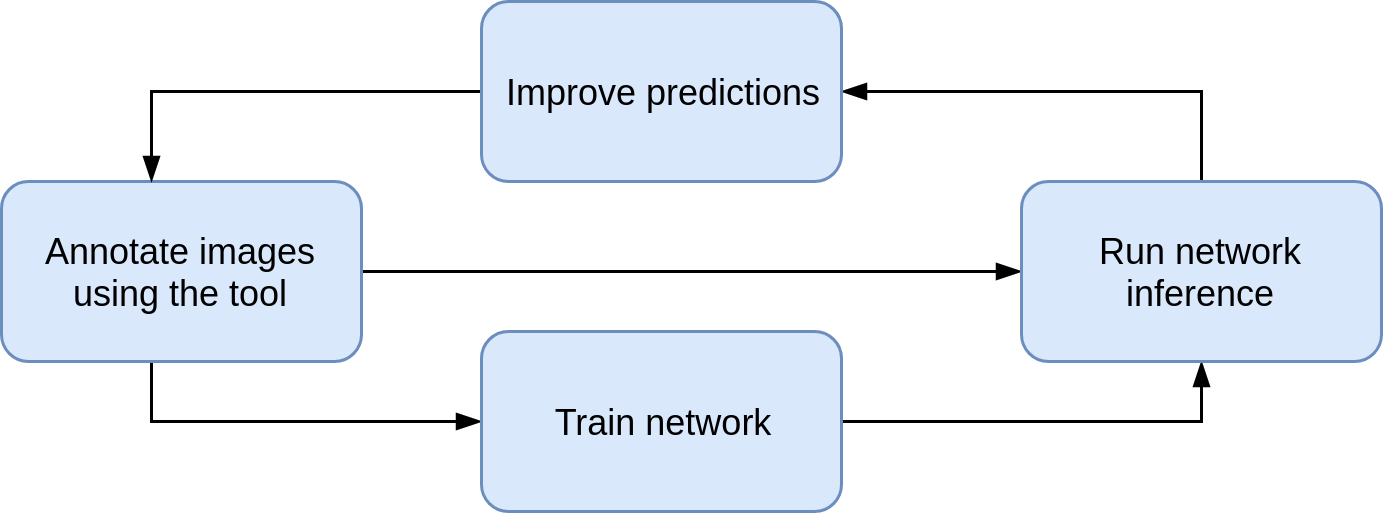
\includegraphics[width=0.75\linewidth]{semi_automatic_workflow}
    \caption{The new workflow of the annotation procedure including the neural network. First, the user has to annotate enough images from the dataset to be able to train the network. After successfully training the network it can be used to predict poses on a subset of the dataset. The user can then improve the poses and return to annotating more images or run the network inference on more images. Own image.}
    	\label{fig:semi_automatic_workflow}
\end{figure}